% =====================================================================
%  THEORY MAP TEMPLATE — Appendix C + Appendix D
%  Reusable across all papers in the Unified Structural Theory
%
%  Author: B. Kriger
%  Last updated: February 2026
%
%  HOW TO USE IN A NEW PAPER:
%
%  1. Copy this file into your project directory.
%
%  2. In your main .tex preamble, ensure you have:
%       \usepackage{tikz}
%       \usetikzlibrary{backgrounds,arrows.meta}
%       \usepackage{geometry}
%       \usepackage{amssymb}
%
%  3. Include this file BEFORE \end{document}:
%       % =====================================================================
%  THEORY MAP TEMPLATE — Appendix C + Appendix D
%  Reusable across all papers in the Unified Structural Theory
%
%  Author: B. Kriger
%  Last updated: February 2026
%
%  HOW TO USE IN A NEW PAPER:
%
%  1. Copy this file into your project directory.
%
%  2. In your main .tex preamble, ensure you have:
%       \usepackage{tikz}
%       \usetikzlibrary{backgrounds,arrows.meta}
%       \usepackage{geometry}
%       \usepackage{amssymb}
%
%  3. Include this file BEFORE \end{document}:
%       % =====================================================================
%  THEORY MAP TEMPLATE — Appendix C + Appendix D
%  Reusable across all papers in the Unified Structural Theory
%
%  Author: B. Kriger
%  Last updated: February 2026
%
%  HOW TO USE IN A NEW PAPER:
%
%  1. Copy this file into your project directory.
%
%  2. In your main .tex preamble, ensure you have:
%       \usepackage{tikz}
%       \usetikzlibrary{backgrounds,arrows.meta}
%       \usepackage{geometry}
%       \usepackage{amssymb}
%
%  3. Include this file BEFORE \end{document}:
%       % =====================================================================
%  THEORY MAP TEMPLATE — Appendix C + Appendix D
%  Reusable across all papers in the Unified Structural Theory
%
%  Author: B. Kriger
%  Last updated: February 2026
%
%  HOW TO USE IN A NEW PAPER:
%
%  1. Copy this file into your project directory.
%
%  2. In your main .tex preamble, ensure you have:
%       \usepackage{tikz}
%       \usetikzlibrary{backgrounds,arrows.meta}
%       \usepackage{geometry}
%       \usepackage{amssymb}
%
%  3. Include this file BEFORE \end{document}:
%       \input{theory_maps_template.tex}
%
%  4. APPENDIX C — Abstract layer map:
%     - Move the "highlight" style to the layer YOUR paper belongs to
%       (currently on Part IV "Social Systems")
%     - Change the \textbf{Dyadic Viability} to YOUR paper's title
%     - Update the caption to describe YOUR paper's dependencies
%
%  5. APPENDIX D — Publication edifice:
%     - Change the \node[H] (the highlighted box) to YOUR paper
%     - If your paper is NEW (not already in the list), add it as
%       a new \node[B] in the appropriate layer and row
%     - Move the $\blacktriangledown$ marker to the new position
%     - Update the total count in the description if needed
%
%  6. When adding a new paper to the edifice, use node style [B]
%     for normal papers and [H] for the current (highlighted) paper.
%     Place it in the correct layer and shift other nodes if needed.
% =====================================================================


% =============================================================
%  APPENDIX C: ABSTRACT SIX-LAYER THEORY MAP
% =============================================================

\clearpage
\section*{Appendix C: Location within the Unified Structural Theory}

\begin{figure}[ht]
\centering
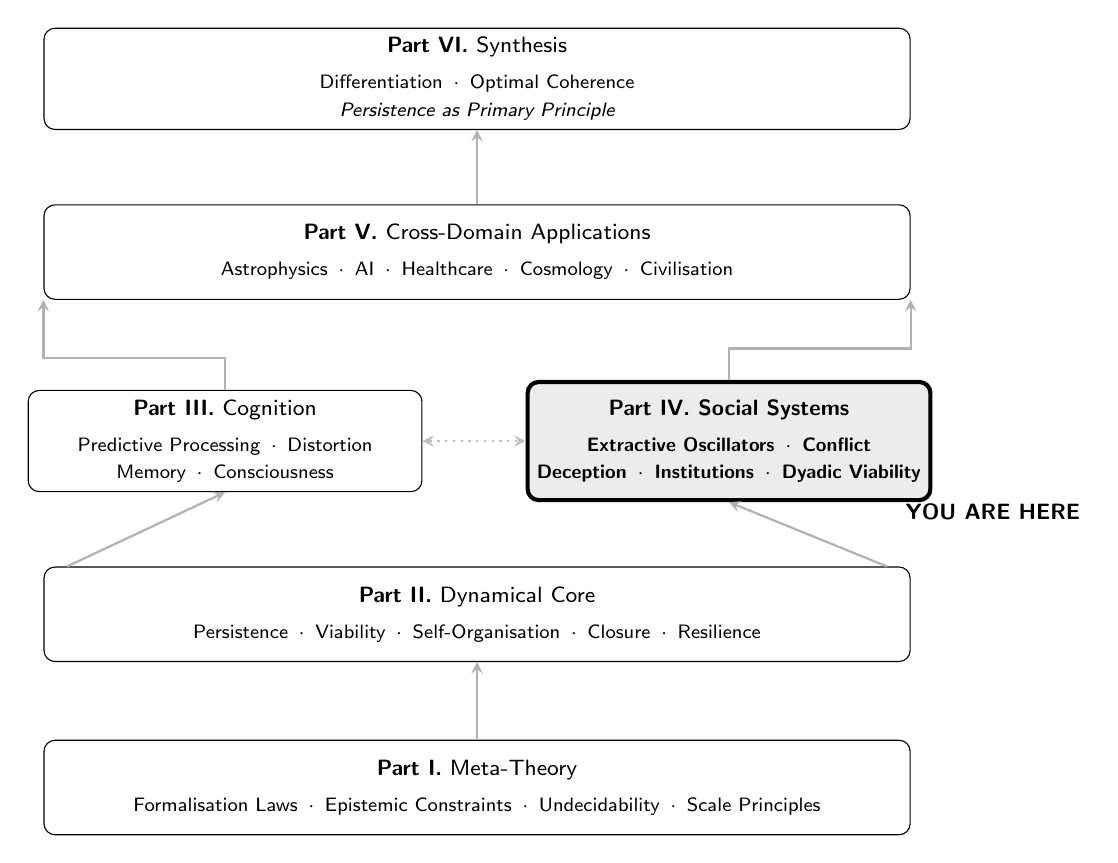
\begin{tikzpicture}[
  every node/.style={font=\sffamily},
  layer/.style={draw, rounded corners=4pt, minimum width=11cm, minimum height=1.2cm, align=center, font=\sffamily\small, fill=white},
  %% --- MOVE "highlight" TO YOUR PAPER'S LAYER ---
  highlight/.style={draw, rounded corners=4pt, minimum width=11cm, minimum height=1.5cm, align=center, font=\sffamily\small\bfseries, fill=gray!15, line width=1.5pt},
  arrow/.style={->, >=stealth, thick, gray!60},
]

% Layer I — Foundation
\node[layer] (meta) at (0, 0) {
  {\footnotesize\textbf{Part I.} Meta-Theory}\\[2pt]
  {\scriptsize Formalisation Laws \,$\cdot$\, Epistemic Constraints \,$\cdot$\, Undecidability \,$\cdot$\, Scale Principles}
};

% Layer II
\node[layer] (core) at (0, 2.2) {
  {\footnotesize\textbf{Part II.} Dynamical Core}\\[2pt]
  {\scriptsize Persistence \,$\cdot$\, Viability \,$\cdot$\, Self-Organisation \,$\cdot$\, Closure \,$\cdot$\, Resilience}
};

% Layer III — Left
\node[layer, minimum width=5cm] (cog) at (-3.2, 4.4) {
  {\footnotesize\textbf{Part III.} Cognition}\\[2pt]
  {\scriptsize Predictive Processing \,$\cdot$\, Distortion}\\[-1pt]
  {\scriptsize Memory \,$\cdot$\, Consciousness}
};

% Layer IV — Right  ← CURRENTLY HIGHLIGHTED (change for your paper)
\node[highlight, minimum width=5cm] (soc) at (3.2, 4.4) {
  {\footnotesize\textbf{Part IV.} Social Systems}\\[2pt]
  {\scriptsize Extractive Oscillators \,$\cdot$\, Conflict}\\[-1pt]
  %% --- CHANGE "Dyadic Viability" TO YOUR PAPER'S SHORT TITLE ---
  {\scriptsize Deception \,$\cdot$\, Institutions \,$\cdot$\, \textbf{Dyadic Viability}}
};

% Marker — move to your layer
\node[font=\sffamily\footnotesize\bfseries] at (6.5, 3.5) {$\blacktriangledown$ YOU ARE HERE};

% Layer V
\node[layer] (app) at (0, 6.8) {
  {\footnotesize\textbf{Part V.} Cross-Domain Applications}\\[2pt]
  {\scriptsize Astrophysics \,$\cdot$\, AI \,$\cdot$\, Healthcare \,$\cdot$\, Cosmology \,$\cdot$\, Civilisation}
};

% Layer VI — Top
\node[layer] (syn) at (0, 9.0) {
  {\footnotesize\textbf{Part VI.} Synthesis}\\[2pt]
  {\scriptsize Differentiation \,$\cdot$\, Optimal Coherence}\\[-1pt]
  {\scriptsize\itshape Persistence as Primary Principle}
};

% Arrows
\draw[arrow] (meta) -- (core);
\draw[arrow] (core.north west) ++(0.3,0) -- (cog.south);
\draw[arrow] (core.north east) ++(-0.3,0) -- (soc.south);
\draw[arrow] (cog.north) -- ++(0, 0.4) -| (app.south west);
\draw[arrow] (soc.north) -- ++(0, 0.4) -| (app.south east);
\draw[arrow] (app) -- (syn);

% Cross-connection
\draw[<->, >=stealth, thick, dotted, gray!50] (cog.east) -- (soc.west);

\end{tikzpicture}
%% --- UPDATE THIS CAPTION FOR YOUR PAPER ---
\caption{Location of the present paper within the Unified Structural Theory of Complex Systems (Kriger, 1999--2026). The theory comprises six layers: foundational meta-theory (I), the dynamical core of structural laws (II), cognitive architecture (III), social systems (IV), cross-domain applications (V), and the overarching synthesis (VI). This paper develops the \emph{Dyadic Viability} model within Part~IV, drawing on the viability, cooperation, and interference laws from Part~II, the structural distortion and extractive oscillator frameworks from Parts~III--IV, and connecting to applications in healthcare, AI, and civilisational analysis in Part~V.}
\label{fig:theory_map}
\end{figure}



% =============================================================
%  APPENDIX D: 76-PAPER PUBLICATION EDIFICE (portrait, 1 page)
% =============================================================
\clearpage
\newgeometry{left=1.2cm, right=1.2cm, top=1.6cm, bottom=0.6cm}

\section*{Appendix D: The Publication Edifice}

\vspace{-1mm}
{\scriptsize All 76 publications (Kriger, 1999--2026) organised bottom-to-top. The present paper is marked~$\blacktriangledown$.}

\vspace{2mm}
\noindent
\resizebox{\textwidth}{!}{%
\begin{tikzpicture}[
  every node/.style={font=\sffamily},
  B/.style={draw, thin, rounded corners=1pt, minimum height=0.6cm, align=left, inner xsep=2pt, inner ysep=1.5pt, font=\sffamily\scriptsize, fill=white, anchor=north west, text width=3.5cm},
  H/.style={draw, line width=1.4pt, rounded corners=2pt, minimum height=0.65cm, align=left, inner xsep=2.5pt, inner ysep=2pt, font=\sffamily\scriptsize\bfseries, fill=black!12, anchor=north west, text width=3.5cm},
  LH/.style={font=\sffamily\scriptsize\bfseries, text=black!45, anchor=south west},
  GA/.style={-{Stealth[length=5pt, width=3.5pt]}, line width=1.4pt, black!30}
]

% 4 columns
\def\cI{0.2}
\def\cII{4.0}
\def\cIII{7.8}
\def\cIV{11.6}
\def\RS{0.88} % row spacing

% ==================================================================
% LAYER I — META-THEORY — 8 papers, 2 rows
% y: 0 to 2.2
% ==================================================================
\fill[black!4, rounded corners=2pt] (0, 0) rectangle (15.3, 2.2);
\node[LH] at (0.1, 2.17) {I\quad META-THEORY};

\node[B] at (\cI,   1.85) {Formalisation Laws (2025)};
\node[B] at (\cII,  1.85) {Imperative Uncertainty (2025)};
\node[B] at (\cIII, 1.85) {Limit to Negation (2025)};
\node[B] at (\cIV,  1.85) {Absurdity as Mercy (2025)};
\node[B] at (\cI,   0.97) {Undecidability as Signal (2023)};
\node[B] at (\cII,  0.97) {No Final Theory: Scale Laws (2024)};
\node[B] at (\cIII, 0.97) {Choice of Formal Realities (2026)};
\node[B] at (\cIV,  0.97) {Def.-Dependent Provability (2026)};

\draw[GA] (7.65, 2.3) -- (7.65, 2.7);

% ==================================================================
% LAYER II — DYNAMICAL CORE — 12 papers, 3 rows
% y: 2.8 to 5.5
% ==================================================================
\fill[black!7, rounded corners=2pt] (0, 2.8) rectangle (15.3, 5.5);
\node[LH] at (0.1, 5.47) {II\quad DYNAMICAL CORE};

\node[B] at (\cI,   5.15) {Four Laws of Self-Org.\ (2017)};
\node[B] at (\cII,  5.15) {Transformational Persistence (2024)};
\node[B] at (\cIII, 5.15) {Structural Resilience (2019)};
\node[B] at (\cIV,  5.15) {Constraint--Autonomy Law (2026)};
\node[B] at (\cI,   4.27) {Viability Mismatch Law (2026)};
\node[B] at (\cII,  4.27) {Newtonian Dynamics Struct.\ (2018)};
\node[B] at (\cIII, 4.27) {Structural Diagnostic Pr.\ (2018)};
\node[B] at (\cIV,  4.27) {Cyclical Hierarchical Syst.\ (2024)};
\node[B] at (\cI,   3.39) {Self-Sufficient Systems (2024)};
\node[B] at (\cII,  3.39) {Assert.--Dismantling Cycles (2015)};
\node[B] at (\cIII, 3.39) {Chaos Is Relative (2026)};
\node[B] at (\cIV,  3.39) {Structural Non-Neutrality (2026)};

\draw[GA] (7.65, 5.6) -- (7.65, 6.0);

% ==================================================================
% LAYER III — COGNITION — 16 papers, 4 rows
% y: 6.1 to 9.7
% ==================================================================
\fill[black!4, rounded corners=2pt] (0, 6.1) rectangle (15.3, 9.7);
\node[LH] at (0.1, 9.67) {III\quad COGNITION};

\node[B] at (\cI,   9.35) {Structural Distortion Pr.\ (2026)};
\node[B] at (\cII,  9.35) {Predictive Processing (2026)};
\node[B] at (\cIII, 9.35) {Representational Isolation (2026)};
\node[B] at (\cIV,  9.35) {Epistemic Constraint Th.\ (2021)};
\node[B] at (\cI,   8.47) {Atemporal Memory (2025)};
\node[B] at (\cII,  8.47) {Evol.\ Sel.\ Atemp.\ Mem.\ (2019)};
\node[B] at (\cIII, 8.47) {Chronoperception Accel.\ (1999)};
\node[B] at (\cIV,  8.47) {Consciousness: Contrad.\ (2021)};
\node[B] at (\cI,   7.59) {Functional Sufficiency (2024)};
\node[B] at (\cII,  7.59) {Operational Term.\ IIT (2024)};
\node[B] at (\cIII, 7.59) {Evol.\ Theory of Credence (2022)};
\node[B] at (\cIV,  7.59) {Reflexive Inference Law (2026)};
\node[B] at (\cI,   6.71) {Mental Disintegration (2026)};
\node[B] at (\cII,  6.71) {Eruptive Manifestation (2026)};
\node[B] at (\cIII, 6.71) {Elim.\ Distortion: Biol.\ Pr.\ (2026)};
\node[B] at (\cIV,  6.71) {Predict.\ Mind: Myth \& Rit.\ (2026)};

\draw[GA] (7.65, 9.8) -- (7.65, 10.2);

% ==================================================================
% LAYER IV — SOCIAL SYSTEMS — 15 papers, 4 rows (4+4+4+3)
% y: 10.3 to 13.9
% ==================================================================
\fill[black!7, rounded corners=2pt] (0, 10.3) rectangle (15.3, 13.9);
\node[LH] at (0.1, 13.87) {IV\quad SOCIAL SYSTEMS};

\node[B] at (\cI,   13.55) {Extractive Oscillators (2017)};
\node[B] at (\cII,  13.55) {Conflict as Phase Trans.\ (2005)};
\node[B] at (\cIII, 13.55) {Deception \& Perc.\ Reality (2025)};
\node[B] at (\cIV,  13.55) {Autonomy Suppression (2020)};
\node[B] at (\cI,   12.67) {Conceptual Responsibility (2014)};
\node[B] at (\cII,  12.67) {Asymm.\ Totalizing Ideals (2026)};
\node[B] at (\cIII, 12.67) {Pre-Integrative Rejection (2026)};
\node[B] at (\cIV,  12.67) {Comparative Asymmetry (2026)};
\node[B] at (\cI,   11.79) {Non-Participation Excl.\ (2026)};
\node[B] at (\cII,  11.79) {Pascal's Wager Dual-Syst.\ (2026)};
\node[B] at (\cIII, 11.79) {Addiction as Extr.\ Osc.\ (2026)};
\node[H] (HERE) at (\cIV, 11.79) {Structural Viability of\\Dyadic Systems (2026)};
\node[B] at (\cI,   10.91) {AI-Extended Communic.\ (2026)};
\node[B] at (\cII,  10.91) {Stimulus Probl.: Post-Sc.\ (2026)};
\node[B] at (\cIII, 10.91) {Inevit.\ Unified Civilis.\ (2026)};

\node[font=\sffamily\small\bfseries, anchor=west] at (15.35, 11.94) {$\blacktriangledown$};

\draw[GA] (7.65, 14.0) -- (7.65, 14.4);

% ==================================================================
% LAYER V — APPLICATIONS — 21 papers, 6 rows
% y: 14.5 to 20.1
% ==================================================================
\fill[black!4, rounded corners=2pt] (0, 14.5) rectangle (15.3, 20.1);
\node[LH] at (0.1, 20.07) {V\quad APPLICATIONS};

\node[font=\sffamily\tiny\itshape, text=black!30, anchor=south west] at (0.2, 19.65) {Astrophysics};
\node[B] at (\cI,   19.55) {Binary-First Star Form.\ (2025)};
\node[B] at (\cII,  19.55) {Why Binary Optimal (2026)};
\node[B] at (\cIII, 19.55) {Swept-Volume Geometry (2026)};
\node[B] at (\cIV,  19.55) {Persist.-Driven Domin.\ (2026)};
\node[B] at (\cI,   18.67) {Protostellar Core Paradox (2026)};
\node[B] at (\cII,  18.67) {Observ.\ Tests VLA/L1551 (2026)};
\node[B] at (\cIII, 18.67) {Can a Star Be Single? (2026)};
\node[B] at (\cIV,  18.67) {Dormant Neutron Stars (2025)};

\node[font=\sffamily\tiny\itshape, text=black!30, anchor=south west] at (0.2, 17.89) {Cosmology \& Methodology};
\node[B] at (\cI,   17.79) {Timescape Cosmology (2025)};
\node[B] at (\cII,  17.79) {Holographic Universe (2025)};
\node[B] at (\cIII, 17.79) {Bayesian Model Comp.\ (2026)};
\node[B] at (\cIV,  17.79) {Struct.-Bayesian Framew.\ (2026)};
\node[B] at (\cI,   16.91) {Ledger Time Model (2025)};

\node[font=\sffamily\tiny\itshape, text=black!30, anchor=south west] at (4.0, 17.13) {Information, AI, Healthcare};
\node[B] at (\cII,  16.91) {Viral Dynamics Framew.\ (2022)};
\node[B] at (\cIII, 16.91) {Quant.\ Clinical Framew.\ (2000)};
\node[B] at (\cIV,  16.91) {Clinical Discont.\ \& AI (2024)};
\node[B] at (\cI,   16.03) {Biospheric Complexity (2026)};
\node[B] at (\cII,  16.03) {Cognitive Syst.\ Compl.\ (2026)};
\node[B] at (\cIII, 16.03) {Local Entropy Inv.\ AI (2026)};
\node[B] at (\cIV,  16.03) {Time Density Dynamics (2026)};
\node[B] at (\cI,   15.15) {Inward Turn: Fermi (2026)};

\draw[GA] (7.65, 20.2) -- (7.65, 20.6);

% ==================================================================
% LAYER VI — SYNTHESIS — 4 papers, 1 row
% y: 20.7 to 21.85
% ==================================================================
\fill[black!7, rounded corners=2pt] (0, 20.7) rectangle (15.3, 21.85);
\node[LH] at (0.1, 21.82) {VI\quad SYNTHESIS};

\node[B] at (\cI,   21.5) {Differentiation as Ontol.\ Cond.\ (2026)};
\node[B] at (\cII,  21.5) {Coherent Syst.\ via Diff.\ (2026)};
\node[B] at (\cIII, 21.5) {Optimal Coherence (2026)};
\node[B] at (\cIV,  21.5) {Inform.\ Preconditions of Meaning (2026)};

% ==================================================================
% APEX
% ==================================================================
\draw[GA] (7.65, 21.95) -- (7.65, 22.35);
\node[draw, thick, rounded corners=3pt, minimum height=0.7cm, align=center, inner sep=5pt,
      font=\sffamily\normalsize\bfseries, fill=black!6, text width=14.8cm, anchor=south west]
  at (0.1, 22.45) {UNIFIED STRUCTURAL THEORY OF COMPLEX SYSTEMS};

\end{tikzpicture}%
}%

\restoregeometry

%
%  4. APPENDIX C — Abstract layer map:
%     - Move the "highlight" style to the layer YOUR paper belongs to
%       (currently on Part IV "Social Systems")
%     - Change the \textbf{Dyadic Viability} to YOUR paper's title
%     - Update the caption to describe YOUR paper's dependencies
%
%  5. APPENDIX D — Publication edifice:
%     - Change the \node[H] (the highlighted box) to YOUR paper
%     - If your paper is NEW (not already in the list), add it as
%       a new \node[B] in the appropriate layer and row
%     - Move the $\blacktriangledown$ marker to the new position
%     - Update the total count in the description if needed
%
%  6. When adding a new paper to the edifice, use node style [B]
%     for normal papers and [H] for the current (highlighted) paper.
%     Place it in the correct layer and shift other nodes if needed.
% =====================================================================


% =============================================================
%  APPENDIX C: ABSTRACT SIX-LAYER THEORY MAP
% =============================================================

\clearpage
\section*{Appendix C: Location within the Unified Structural Theory}

\begin{figure}[ht]
\centering
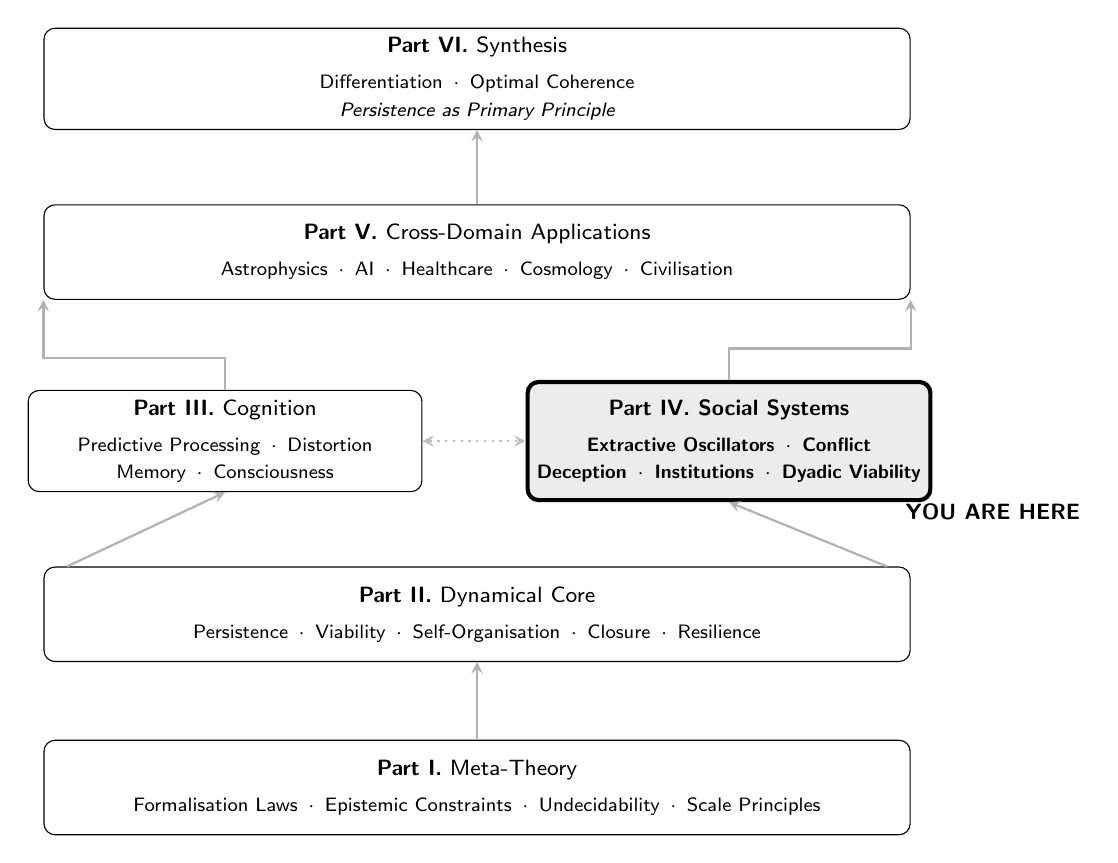
\begin{tikzpicture}[
  every node/.style={font=\sffamily},
  layer/.style={draw, rounded corners=4pt, minimum width=11cm, minimum height=1.2cm, align=center, font=\sffamily\small, fill=white},
  %% --- MOVE "highlight" TO YOUR PAPER'S LAYER ---
  highlight/.style={draw, rounded corners=4pt, minimum width=11cm, minimum height=1.5cm, align=center, font=\sffamily\small\bfseries, fill=gray!15, line width=1.5pt},
  arrow/.style={->, >=stealth, thick, gray!60},
]

% Layer I — Foundation
\node[layer] (meta) at (0, 0) {
  {\footnotesize\textbf{Part I.} Meta-Theory}\\[2pt]
  {\scriptsize Formalisation Laws \,$\cdot$\, Epistemic Constraints \,$\cdot$\, Undecidability \,$\cdot$\, Scale Principles}
};

% Layer II
\node[layer] (core) at (0, 2.2) {
  {\footnotesize\textbf{Part II.} Dynamical Core}\\[2pt]
  {\scriptsize Persistence \,$\cdot$\, Viability \,$\cdot$\, Self-Organisation \,$\cdot$\, Closure \,$\cdot$\, Resilience}
};

% Layer III — Left
\node[layer, minimum width=5cm] (cog) at (-3.2, 4.4) {
  {\footnotesize\textbf{Part III.} Cognition}\\[2pt]
  {\scriptsize Predictive Processing \,$\cdot$\, Distortion}\\[-1pt]
  {\scriptsize Memory \,$\cdot$\, Consciousness}
};

% Layer IV — Right  ← CURRENTLY HIGHLIGHTED (change for your paper)
\node[highlight, minimum width=5cm] (soc) at (3.2, 4.4) {
  {\footnotesize\textbf{Part IV.} Social Systems}\\[2pt]
  {\scriptsize Extractive Oscillators \,$\cdot$\, Conflict}\\[-1pt]
  %% --- CHANGE "Dyadic Viability" TO YOUR PAPER'S SHORT TITLE ---
  {\scriptsize Deception \,$\cdot$\, Institutions \,$\cdot$\, \textbf{Dyadic Viability}}
};

% Marker — move to your layer
\node[font=\sffamily\footnotesize\bfseries] at (6.5, 3.5) {$\blacktriangledown$ YOU ARE HERE};

% Layer V
\node[layer] (app) at (0, 6.8) {
  {\footnotesize\textbf{Part V.} Cross-Domain Applications}\\[2pt]
  {\scriptsize Astrophysics \,$\cdot$\, AI \,$\cdot$\, Healthcare \,$\cdot$\, Cosmology \,$\cdot$\, Civilisation}
};

% Layer VI — Top
\node[layer] (syn) at (0, 9.0) {
  {\footnotesize\textbf{Part VI.} Synthesis}\\[2pt]
  {\scriptsize Differentiation \,$\cdot$\, Optimal Coherence}\\[-1pt]
  {\scriptsize\itshape Persistence as Primary Principle}
};

% Arrows
\draw[arrow] (meta) -- (core);
\draw[arrow] (core.north west) ++(0.3,0) -- (cog.south);
\draw[arrow] (core.north east) ++(-0.3,0) -- (soc.south);
\draw[arrow] (cog.north) -- ++(0, 0.4) -| (app.south west);
\draw[arrow] (soc.north) -- ++(0, 0.4) -| (app.south east);
\draw[arrow] (app) -- (syn);

% Cross-connection
\draw[<->, >=stealth, thick, dotted, gray!50] (cog.east) -- (soc.west);

\end{tikzpicture}
%% --- UPDATE THIS CAPTION FOR YOUR PAPER ---
\caption{Location of the present paper within the Unified Structural Theory of Complex Systems (Kriger, 1999--2026). The theory comprises six layers: foundational meta-theory (I), the dynamical core of structural laws (II), cognitive architecture (III), social systems (IV), cross-domain applications (V), and the overarching synthesis (VI). This paper develops the \emph{Dyadic Viability} model within Part~IV, drawing on the viability, cooperation, and interference laws from Part~II, the structural distortion and extractive oscillator frameworks from Parts~III--IV, and connecting to applications in healthcare, AI, and civilisational analysis in Part~V.}
\label{fig:theory_map}
\end{figure}



% =============================================================
%  APPENDIX D: 76-PAPER PUBLICATION EDIFICE (portrait, 1 page)
% =============================================================
\clearpage
\newgeometry{left=1.2cm, right=1.2cm, top=1.6cm, bottom=0.6cm}

\section*{Appendix D: The Publication Edifice}

\vspace{-1mm}
{\scriptsize All 76 publications (Kriger, 1999--2026) organised bottom-to-top. The present paper is marked~$\blacktriangledown$.}

\vspace{2mm}
\noindent
\resizebox{\textwidth}{!}{%
\begin{tikzpicture}[
  every node/.style={font=\sffamily},
  B/.style={draw, thin, rounded corners=1pt, minimum height=0.6cm, align=left, inner xsep=2pt, inner ysep=1.5pt, font=\sffamily\scriptsize, fill=white, anchor=north west, text width=3.5cm},
  H/.style={draw, line width=1.4pt, rounded corners=2pt, minimum height=0.65cm, align=left, inner xsep=2.5pt, inner ysep=2pt, font=\sffamily\scriptsize\bfseries, fill=black!12, anchor=north west, text width=3.5cm},
  LH/.style={font=\sffamily\scriptsize\bfseries, text=black!45, anchor=south west},
  GA/.style={-{Stealth[length=5pt, width=3.5pt]}, line width=1.4pt, black!30}
]

% 4 columns
\def\cI{0.2}
\def\cII{4.0}
\def\cIII{7.8}
\def\cIV{11.6}
\def\RS{0.88} % row spacing

% ==================================================================
% LAYER I — META-THEORY — 8 papers, 2 rows
% y: 0 to 2.2
% ==================================================================
\fill[black!4, rounded corners=2pt] (0, 0) rectangle (15.3, 2.2);
\node[LH] at (0.1, 2.17) {I\quad META-THEORY};

\node[B] at (\cI,   1.85) {Formalisation Laws (2025)};
\node[B] at (\cII,  1.85) {Imperative Uncertainty (2025)};
\node[B] at (\cIII, 1.85) {Limit to Negation (2025)};
\node[B] at (\cIV,  1.85) {Absurdity as Mercy (2025)};
\node[B] at (\cI,   0.97) {Undecidability as Signal (2023)};
\node[B] at (\cII,  0.97) {No Final Theory: Scale Laws (2024)};
\node[B] at (\cIII, 0.97) {Choice of Formal Realities (2026)};
\node[B] at (\cIV,  0.97) {Def.-Dependent Provability (2026)};

\draw[GA] (7.65, 2.3) -- (7.65, 2.7);

% ==================================================================
% LAYER II — DYNAMICAL CORE — 12 papers, 3 rows
% y: 2.8 to 5.5
% ==================================================================
\fill[black!7, rounded corners=2pt] (0, 2.8) rectangle (15.3, 5.5);
\node[LH] at (0.1, 5.47) {II\quad DYNAMICAL CORE};

\node[B] at (\cI,   5.15) {Four Laws of Self-Org.\ (2017)};
\node[B] at (\cII,  5.15) {Transformational Persistence (2024)};
\node[B] at (\cIII, 5.15) {Structural Resilience (2019)};
\node[B] at (\cIV,  5.15) {Constraint--Autonomy Law (2026)};
\node[B] at (\cI,   4.27) {Viability Mismatch Law (2026)};
\node[B] at (\cII,  4.27) {Newtonian Dynamics Struct.\ (2018)};
\node[B] at (\cIII, 4.27) {Structural Diagnostic Pr.\ (2018)};
\node[B] at (\cIV,  4.27) {Cyclical Hierarchical Syst.\ (2024)};
\node[B] at (\cI,   3.39) {Self-Sufficient Systems (2024)};
\node[B] at (\cII,  3.39) {Assert.--Dismantling Cycles (2015)};
\node[B] at (\cIII, 3.39) {Chaos Is Relative (2026)};
\node[B] at (\cIV,  3.39) {Structural Non-Neutrality (2026)};

\draw[GA] (7.65, 5.6) -- (7.65, 6.0);

% ==================================================================
% LAYER III — COGNITION — 16 papers, 4 rows
% y: 6.1 to 9.7
% ==================================================================
\fill[black!4, rounded corners=2pt] (0, 6.1) rectangle (15.3, 9.7);
\node[LH] at (0.1, 9.67) {III\quad COGNITION};

\node[B] at (\cI,   9.35) {Structural Distortion Pr.\ (2026)};
\node[B] at (\cII,  9.35) {Predictive Processing (2026)};
\node[B] at (\cIII, 9.35) {Representational Isolation (2026)};
\node[B] at (\cIV,  9.35) {Epistemic Constraint Th.\ (2021)};
\node[B] at (\cI,   8.47) {Atemporal Memory (2025)};
\node[B] at (\cII,  8.47) {Evol.\ Sel.\ Atemp.\ Mem.\ (2019)};
\node[B] at (\cIII, 8.47) {Chronoperception Accel.\ (1999)};
\node[B] at (\cIV,  8.47) {Consciousness: Contrad.\ (2021)};
\node[B] at (\cI,   7.59) {Functional Sufficiency (2024)};
\node[B] at (\cII,  7.59) {Operational Term.\ IIT (2024)};
\node[B] at (\cIII, 7.59) {Evol.\ Theory of Credence (2022)};
\node[B] at (\cIV,  7.59) {Reflexive Inference Law (2026)};
\node[B] at (\cI,   6.71) {Mental Disintegration (2026)};
\node[B] at (\cII,  6.71) {Eruptive Manifestation (2026)};
\node[B] at (\cIII, 6.71) {Elim.\ Distortion: Biol.\ Pr.\ (2026)};
\node[B] at (\cIV,  6.71) {Predict.\ Mind: Myth \& Rit.\ (2026)};

\draw[GA] (7.65, 9.8) -- (7.65, 10.2);

% ==================================================================
% LAYER IV — SOCIAL SYSTEMS — 15 papers, 4 rows (4+4+4+3)
% y: 10.3 to 13.9
% ==================================================================
\fill[black!7, rounded corners=2pt] (0, 10.3) rectangle (15.3, 13.9);
\node[LH] at (0.1, 13.87) {IV\quad SOCIAL SYSTEMS};

\node[B] at (\cI,   13.55) {Extractive Oscillators (2017)};
\node[B] at (\cII,  13.55) {Conflict as Phase Trans.\ (2005)};
\node[B] at (\cIII, 13.55) {Deception \& Perc.\ Reality (2025)};
\node[B] at (\cIV,  13.55) {Autonomy Suppression (2020)};
\node[B] at (\cI,   12.67) {Conceptual Responsibility (2014)};
\node[B] at (\cII,  12.67) {Asymm.\ Totalizing Ideals (2026)};
\node[B] at (\cIII, 12.67) {Pre-Integrative Rejection (2026)};
\node[B] at (\cIV,  12.67) {Comparative Asymmetry (2026)};
\node[B] at (\cI,   11.79) {Non-Participation Excl.\ (2026)};
\node[B] at (\cII,  11.79) {Pascal's Wager Dual-Syst.\ (2026)};
\node[B] at (\cIII, 11.79) {Addiction as Extr.\ Osc.\ (2026)};
\node[H] (HERE) at (\cIV, 11.79) {Structural Viability of\\Dyadic Systems (2026)};
\node[B] at (\cI,   10.91) {AI-Extended Communic.\ (2026)};
\node[B] at (\cII,  10.91) {Stimulus Probl.: Post-Sc.\ (2026)};
\node[B] at (\cIII, 10.91) {Inevit.\ Unified Civilis.\ (2026)};

\node[font=\sffamily\small\bfseries, anchor=west] at (15.35, 11.94) {$\blacktriangledown$};

\draw[GA] (7.65, 14.0) -- (7.65, 14.4);

% ==================================================================
% LAYER V — APPLICATIONS — 21 papers, 6 rows
% y: 14.5 to 20.1
% ==================================================================
\fill[black!4, rounded corners=2pt] (0, 14.5) rectangle (15.3, 20.1);
\node[LH] at (0.1, 20.07) {V\quad APPLICATIONS};

\node[font=\sffamily\tiny\itshape, text=black!30, anchor=south west] at (0.2, 19.65) {Astrophysics};
\node[B] at (\cI,   19.55) {Binary-First Star Form.\ (2025)};
\node[B] at (\cII,  19.55) {Why Binary Optimal (2026)};
\node[B] at (\cIII, 19.55) {Swept-Volume Geometry (2026)};
\node[B] at (\cIV,  19.55) {Persist.-Driven Domin.\ (2026)};
\node[B] at (\cI,   18.67) {Protostellar Core Paradox (2026)};
\node[B] at (\cII,  18.67) {Observ.\ Tests VLA/L1551 (2026)};
\node[B] at (\cIII, 18.67) {Can a Star Be Single? (2026)};
\node[B] at (\cIV,  18.67) {Dormant Neutron Stars (2025)};

\node[font=\sffamily\tiny\itshape, text=black!30, anchor=south west] at (0.2, 17.89) {Cosmology \& Methodology};
\node[B] at (\cI,   17.79) {Timescape Cosmology (2025)};
\node[B] at (\cII,  17.79) {Holographic Universe (2025)};
\node[B] at (\cIII, 17.79) {Bayesian Model Comp.\ (2026)};
\node[B] at (\cIV,  17.79) {Struct.-Bayesian Framew.\ (2026)};
\node[B] at (\cI,   16.91) {Ledger Time Model (2025)};

\node[font=\sffamily\tiny\itshape, text=black!30, anchor=south west] at (4.0, 17.13) {Information, AI, Healthcare};
\node[B] at (\cII,  16.91) {Viral Dynamics Framew.\ (2022)};
\node[B] at (\cIII, 16.91) {Quant.\ Clinical Framew.\ (2000)};
\node[B] at (\cIV,  16.91) {Clinical Discont.\ \& AI (2024)};
\node[B] at (\cI,   16.03) {Biospheric Complexity (2026)};
\node[B] at (\cII,  16.03) {Cognitive Syst.\ Compl.\ (2026)};
\node[B] at (\cIII, 16.03) {Local Entropy Inv.\ AI (2026)};
\node[B] at (\cIV,  16.03) {Time Density Dynamics (2026)};
\node[B] at (\cI,   15.15) {Inward Turn: Fermi (2026)};

\draw[GA] (7.65, 20.2) -- (7.65, 20.6);

% ==================================================================
% LAYER VI — SYNTHESIS — 4 papers, 1 row
% y: 20.7 to 21.85
% ==================================================================
\fill[black!7, rounded corners=2pt] (0, 20.7) rectangle (15.3, 21.85);
\node[LH] at (0.1, 21.82) {VI\quad SYNTHESIS};

\node[B] at (\cI,   21.5) {Differentiation as Ontol.\ Cond.\ (2026)};
\node[B] at (\cII,  21.5) {Coherent Syst.\ via Diff.\ (2026)};
\node[B] at (\cIII, 21.5) {Optimal Coherence (2026)};
\node[B] at (\cIV,  21.5) {Inform.\ Preconditions of Meaning (2026)};

% ==================================================================
% APEX
% ==================================================================
\draw[GA] (7.65, 21.95) -- (7.65, 22.35);
\node[draw, thick, rounded corners=3pt, minimum height=0.7cm, align=center, inner sep=5pt,
      font=\sffamily\normalsize\bfseries, fill=black!6, text width=14.8cm, anchor=south west]
  at (0.1, 22.45) {UNIFIED STRUCTURAL THEORY OF COMPLEX SYSTEMS};

\end{tikzpicture}%
}%

\restoregeometry

%
%  4. APPENDIX C — Abstract layer map:
%     - Move the "highlight" style to the layer YOUR paper belongs to
%       (currently on Part IV "Social Systems")
%     - Change the \textbf{Dyadic Viability} to YOUR paper's title
%     - Update the caption to describe YOUR paper's dependencies
%
%  5. APPENDIX D — Publication edifice:
%     - Change the \node[H] (the highlighted box) to YOUR paper
%     - If your paper is NEW (not already in the list), add it as
%       a new \node[B] in the appropriate layer and row
%     - Move the $\blacktriangledown$ marker to the new position
%     - Update the total count in the description if needed
%
%  6. When adding a new paper to the edifice, use node style [B]
%     for normal papers and [H] for the current (highlighted) paper.
%     Place it in the correct layer and shift other nodes if needed.
% =====================================================================


% =============================================================
%  APPENDIX C: ABSTRACT SIX-LAYER THEORY MAP
% =============================================================

\clearpage
\section*{Appendix C: Location within the Unified Structural Theory}

\begin{figure}[ht]
\centering
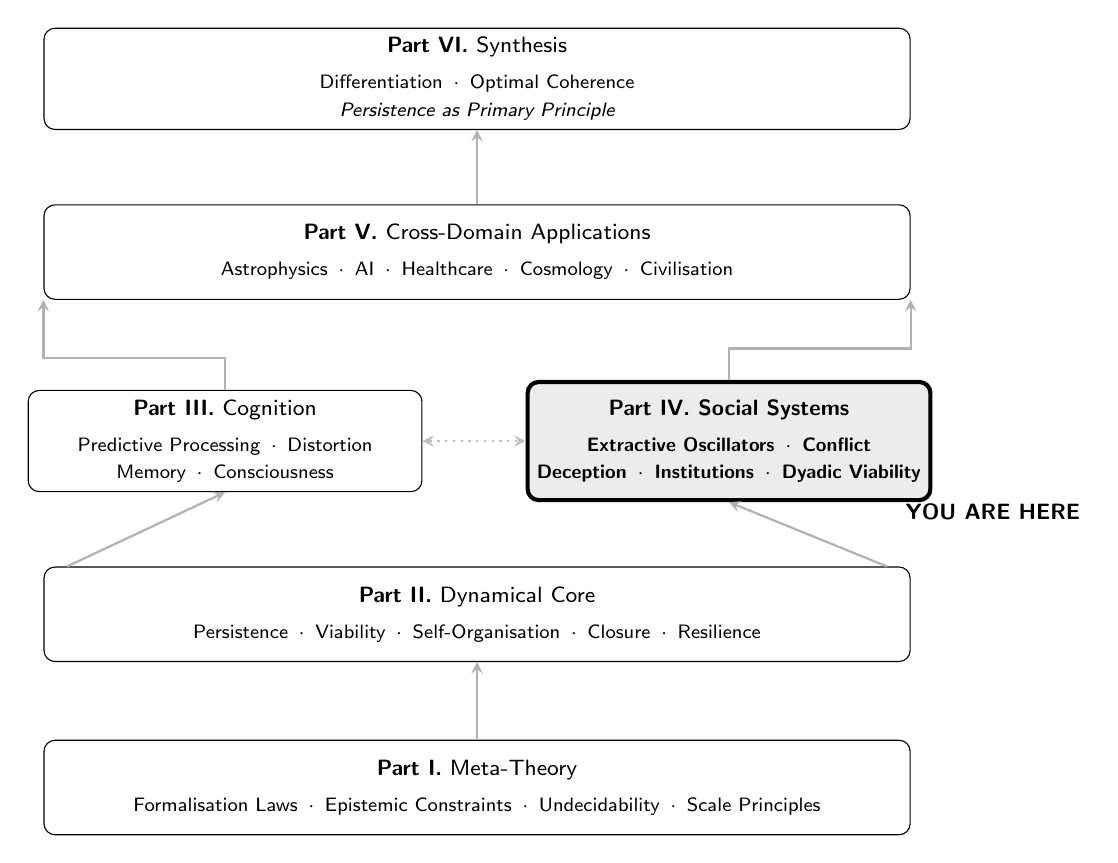
\begin{tikzpicture}[
  every node/.style={font=\sffamily},
  layer/.style={draw, rounded corners=4pt, minimum width=11cm, minimum height=1.2cm, align=center, font=\sffamily\small, fill=white},
  %% --- MOVE "highlight" TO YOUR PAPER'S LAYER ---
  highlight/.style={draw, rounded corners=4pt, minimum width=11cm, minimum height=1.5cm, align=center, font=\sffamily\small\bfseries, fill=gray!15, line width=1.5pt},
  arrow/.style={->, >=stealth, thick, gray!60},
]

% Layer I — Foundation
\node[layer] (meta) at (0, 0) {
  {\footnotesize\textbf{Part I.} Meta-Theory}\\[2pt]
  {\scriptsize Formalisation Laws \,$\cdot$\, Epistemic Constraints \,$\cdot$\, Undecidability \,$\cdot$\, Scale Principles}
};

% Layer II
\node[layer] (core) at (0, 2.2) {
  {\footnotesize\textbf{Part II.} Dynamical Core}\\[2pt]
  {\scriptsize Persistence \,$\cdot$\, Viability \,$\cdot$\, Self-Organisation \,$\cdot$\, Closure \,$\cdot$\, Resilience}
};

% Layer III — Left
\node[layer, minimum width=5cm] (cog) at (-3.2, 4.4) {
  {\footnotesize\textbf{Part III.} Cognition}\\[2pt]
  {\scriptsize Predictive Processing \,$\cdot$\, Distortion}\\[-1pt]
  {\scriptsize Memory \,$\cdot$\, Consciousness}
};

% Layer IV — Right  ← CURRENTLY HIGHLIGHTED (change for your paper)
\node[highlight, minimum width=5cm] (soc) at (3.2, 4.4) {
  {\footnotesize\textbf{Part IV.} Social Systems}\\[2pt]
  {\scriptsize Extractive Oscillators \,$\cdot$\, Conflict}\\[-1pt]
  %% --- CHANGE "Dyadic Viability" TO YOUR PAPER'S SHORT TITLE ---
  {\scriptsize Deception \,$\cdot$\, Institutions \,$\cdot$\, \textbf{Dyadic Viability}}
};

% Marker — move to your layer
\node[font=\sffamily\footnotesize\bfseries] at (6.5, 3.5) {$\blacktriangledown$ YOU ARE HERE};

% Layer V
\node[layer] (app) at (0, 6.8) {
  {\footnotesize\textbf{Part V.} Cross-Domain Applications}\\[2pt]
  {\scriptsize Astrophysics \,$\cdot$\, AI \,$\cdot$\, Healthcare \,$\cdot$\, Cosmology \,$\cdot$\, Civilisation}
};

% Layer VI — Top
\node[layer] (syn) at (0, 9.0) {
  {\footnotesize\textbf{Part VI.} Synthesis}\\[2pt]
  {\scriptsize Differentiation \,$\cdot$\, Optimal Coherence}\\[-1pt]
  {\scriptsize\itshape Persistence as Primary Principle}
};

% Arrows
\draw[arrow] (meta) -- (core);
\draw[arrow] (core.north west) ++(0.3,0) -- (cog.south);
\draw[arrow] (core.north east) ++(-0.3,0) -- (soc.south);
\draw[arrow] (cog.north) -- ++(0, 0.4) -| (app.south west);
\draw[arrow] (soc.north) -- ++(0, 0.4) -| (app.south east);
\draw[arrow] (app) -- (syn);

% Cross-connection
\draw[<->, >=stealth, thick, dotted, gray!50] (cog.east) -- (soc.west);

\end{tikzpicture}
%% --- UPDATE THIS CAPTION FOR YOUR PAPER ---
\caption{Location of the present paper within the Unified Structural Theory of Complex Systems (Kriger, 1999--2026). The theory comprises six layers: foundational meta-theory (I), the dynamical core of structural laws (II), cognitive architecture (III), social systems (IV), cross-domain applications (V), and the overarching synthesis (VI). This paper develops the \emph{Dyadic Viability} model within Part~IV, drawing on the viability, cooperation, and interference laws from Part~II, the structural distortion and extractive oscillator frameworks from Parts~III--IV, and connecting to applications in healthcare, AI, and civilisational analysis in Part~V.}
\label{fig:theory_map}
\end{figure}



% =============================================================
%  APPENDIX D: 76-PAPER PUBLICATION EDIFICE (portrait, 1 page)
% =============================================================
\clearpage
\newgeometry{left=1.2cm, right=1.2cm, top=1.6cm, bottom=0.6cm}

\section*{Appendix D: The Publication Edifice}

\vspace{-1mm}
{\scriptsize All 76 publications (Kriger, 1999--2026) organised bottom-to-top. The present paper is marked~$\blacktriangledown$.}

\vspace{2mm}
\noindent
\resizebox{\textwidth}{!}{%
\begin{tikzpicture}[
  every node/.style={font=\sffamily},
  B/.style={draw, thin, rounded corners=1pt, minimum height=0.6cm, align=left, inner xsep=2pt, inner ysep=1.5pt, font=\sffamily\scriptsize, fill=white, anchor=north west, text width=3.5cm},
  H/.style={draw, line width=1.4pt, rounded corners=2pt, minimum height=0.65cm, align=left, inner xsep=2.5pt, inner ysep=2pt, font=\sffamily\scriptsize\bfseries, fill=black!12, anchor=north west, text width=3.5cm},
  LH/.style={font=\sffamily\scriptsize\bfseries, text=black!45, anchor=south west},
  GA/.style={-{Stealth[length=5pt, width=3.5pt]}, line width=1.4pt, black!30}
]

% 4 columns
\def\cI{0.2}
\def\cII{4.0}
\def\cIII{7.8}
\def\cIV{11.6}
\def\RS{0.88} % row spacing

% ==================================================================
% LAYER I — META-THEORY — 8 papers, 2 rows
% y: 0 to 2.2
% ==================================================================
\fill[black!4, rounded corners=2pt] (0, 0) rectangle (15.3, 2.2);
\node[LH] at (0.1, 2.17) {I\quad META-THEORY};

\node[B] at (\cI,   1.85) {Formalisation Laws (2025)};
\node[B] at (\cII,  1.85) {Imperative Uncertainty (2025)};
\node[B] at (\cIII, 1.85) {Limit to Negation (2025)};
\node[B] at (\cIV,  1.85) {Absurdity as Mercy (2025)};
\node[B] at (\cI,   0.97) {Undecidability as Signal (2023)};
\node[B] at (\cII,  0.97) {No Final Theory: Scale Laws (2024)};
\node[B] at (\cIII, 0.97) {Choice of Formal Realities (2026)};
\node[B] at (\cIV,  0.97) {Def.-Dependent Provability (2026)};

\draw[GA] (7.65, 2.3) -- (7.65, 2.7);

% ==================================================================
% LAYER II — DYNAMICAL CORE — 12 papers, 3 rows
% y: 2.8 to 5.5
% ==================================================================
\fill[black!7, rounded corners=2pt] (0, 2.8) rectangle (15.3, 5.5);
\node[LH] at (0.1, 5.47) {II\quad DYNAMICAL CORE};

\node[B] at (\cI,   5.15) {Four Laws of Self-Org.\ (2017)};
\node[B] at (\cII,  5.15) {Transformational Persistence (2024)};
\node[B] at (\cIII, 5.15) {Structural Resilience (2019)};
\node[B] at (\cIV,  5.15) {Constraint--Autonomy Law (2026)};
\node[B] at (\cI,   4.27) {Viability Mismatch Law (2026)};
\node[B] at (\cII,  4.27) {Newtonian Dynamics Struct.\ (2018)};
\node[B] at (\cIII, 4.27) {Structural Diagnostic Pr.\ (2018)};
\node[B] at (\cIV,  4.27) {Cyclical Hierarchical Syst.\ (2024)};
\node[B] at (\cI,   3.39) {Self-Sufficient Systems (2024)};
\node[B] at (\cII,  3.39) {Assert.--Dismantling Cycles (2015)};
\node[B] at (\cIII, 3.39) {Chaos Is Relative (2026)};
\node[B] at (\cIV,  3.39) {Structural Non-Neutrality (2026)};

\draw[GA] (7.65, 5.6) -- (7.65, 6.0);

% ==================================================================
% LAYER III — COGNITION — 16 papers, 4 rows
% y: 6.1 to 9.7
% ==================================================================
\fill[black!4, rounded corners=2pt] (0, 6.1) rectangle (15.3, 9.7);
\node[LH] at (0.1, 9.67) {III\quad COGNITION};

\node[B] at (\cI,   9.35) {Structural Distortion Pr.\ (2026)};
\node[B] at (\cII,  9.35) {Predictive Processing (2026)};
\node[B] at (\cIII, 9.35) {Representational Isolation (2026)};
\node[B] at (\cIV,  9.35) {Epistemic Constraint Th.\ (2021)};
\node[B] at (\cI,   8.47) {Atemporal Memory (2025)};
\node[B] at (\cII,  8.47) {Evol.\ Sel.\ Atemp.\ Mem.\ (2019)};
\node[B] at (\cIII, 8.47) {Chronoperception Accel.\ (1999)};
\node[B] at (\cIV,  8.47) {Consciousness: Contrad.\ (2021)};
\node[B] at (\cI,   7.59) {Functional Sufficiency (2024)};
\node[B] at (\cII,  7.59) {Operational Term.\ IIT (2024)};
\node[B] at (\cIII, 7.59) {Evol.\ Theory of Credence (2022)};
\node[B] at (\cIV,  7.59) {Reflexive Inference Law (2026)};
\node[B] at (\cI,   6.71) {Mental Disintegration (2026)};
\node[B] at (\cII,  6.71) {Eruptive Manifestation (2026)};
\node[B] at (\cIII, 6.71) {Elim.\ Distortion: Biol.\ Pr.\ (2026)};
\node[B] at (\cIV,  6.71) {Predict.\ Mind: Myth \& Rit.\ (2026)};

\draw[GA] (7.65, 9.8) -- (7.65, 10.2);

% ==================================================================
% LAYER IV — SOCIAL SYSTEMS — 15 papers, 4 rows (4+4+4+3)
% y: 10.3 to 13.9
% ==================================================================
\fill[black!7, rounded corners=2pt] (0, 10.3) rectangle (15.3, 13.9);
\node[LH] at (0.1, 13.87) {IV\quad SOCIAL SYSTEMS};

\node[B] at (\cI,   13.55) {Extractive Oscillators (2017)};
\node[B] at (\cII,  13.55) {Conflict as Phase Trans.\ (2005)};
\node[B] at (\cIII, 13.55) {Deception \& Perc.\ Reality (2025)};
\node[B] at (\cIV,  13.55) {Autonomy Suppression (2020)};
\node[B] at (\cI,   12.67) {Conceptual Responsibility (2014)};
\node[B] at (\cII,  12.67) {Asymm.\ Totalizing Ideals (2026)};
\node[B] at (\cIII, 12.67) {Pre-Integrative Rejection (2026)};
\node[B] at (\cIV,  12.67) {Comparative Asymmetry (2026)};
\node[B] at (\cI,   11.79) {Non-Participation Excl.\ (2026)};
\node[B] at (\cII,  11.79) {Pascal's Wager Dual-Syst.\ (2026)};
\node[B] at (\cIII, 11.79) {Addiction as Extr.\ Osc.\ (2026)};
\node[H] (HERE) at (\cIV, 11.79) {Structural Viability of\\Dyadic Systems (2026)};
\node[B] at (\cI,   10.91) {AI-Extended Communic.\ (2026)};
\node[B] at (\cII,  10.91) {Stimulus Probl.: Post-Sc.\ (2026)};
\node[B] at (\cIII, 10.91) {Inevit.\ Unified Civilis.\ (2026)};

\node[font=\sffamily\small\bfseries, anchor=west] at (15.35, 11.94) {$\blacktriangledown$};

\draw[GA] (7.65, 14.0) -- (7.65, 14.4);

% ==================================================================
% LAYER V — APPLICATIONS — 21 papers, 6 rows
% y: 14.5 to 20.1
% ==================================================================
\fill[black!4, rounded corners=2pt] (0, 14.5) rectangle (15.3, 20.1);
\node[LH] at (0.1, 20.07) {V\quad APPLICATIONS};

\node[font=\sffamily\tiny\itshape, text=black!30, anchor=south west] at (0.2, 19.65) {Astrophysics};
\node[B] at (\cI,   19.55) {Binary-First Star Form.\ (2025)};
\node[B] at (\cII,  19.55) {Why Binary Optimal (2026)};
\node[B] at (\cIII, 19.55) {Swept-Volume Geometry (2026)};
\node[B] at (\cIV,  19.55) {Persist.-Driven Domin.\ (2026)};
\node[B] at (\cI,   18.67) {Protostellar Core Paradox (2026)};
\node[B] at (\cII,  18.67) {Observ.\ Tests VLA/L1551 (2026)};
\node[B] at (\cIII, 18.67) {Can a Star Be Single? (2026)};
\node[B] at (\cIV,  18.67) {Dormant Neutron Stars (2025)};

\node[font=\sffamily\tiny\itshape, text=black!30, anchor=south west] at (0.2, 17.89) {Cosmology \& Methodology};
\node[B] at (\cI,   17.79) {Timescape Cosmology (2025)};
\node[B] at (\cII,  17.79) {Holographic Universe (2025)};
\node[B] at (\cIII, 17.79) {Bayesian Model Comp.\ (2026)};
\node[B] at (\cIV,  17.79) {Struct.-Bayesian Framew.\ (2026)};
\node[B] at (\cI,   16.91) {Ledger Time Model (2025)};

\node[font=\sffamily\tiny\itshape, text=black!30, anchor=south west] at (4.0, 17.13) {Information, AI, Healthcare};
\node[B] at (\cII,  16.91) {Viral Dynamics Framew.\ (2022)};
\node[B] at (\cIII, 16.91) {Quant.\ Clinical Framew.\ (2000)};
\node[B] at (\cIV,  16.91) {Clinical Discont.\ \& AI (2024)};
\node[B] at (\cI,   16.03) {Biospheric Complexity (2026)};
\node[B] at (\cII,  16.03) {Cognitive Syst.\ Compl.\ (2026)};
\node[B] at (\cIII, 16.03) {Local Entropy Inv.\ AI (2026)};
\node[B] at (\cIV,  16.03) {Time Density Dynamics (2026)};
\node[B] at (\cI,   15.15) {Inward Turn: Fermi (2026)};

\draw[GA] (7.65, 20.2) -- (7.65, 20.6);

% ==================================================================
% LAYER VI — SYNTHESIS — 4 papers, 1 row
% y: 20.7 to 21.85
% ==================================================================
\fill[black!7, rounded corners=2pt] (0, 20.7) rectangle (15.3, 21.85);
\node[LH] at (0.1, 21.82) {VI\quad SYNTHESIS};

\node[B] at (\cI,   21.5) {Differentiation as Ontol.\ Cond.\ (2026)};
\node[B] at (\cII,  21.5) {Coherent Syst.\ via Diff.\ (2026)};
\node[B] at (\cIII, 21.5) {Optimal Coherence (2026)};
\node[B] at (\cIV,  21.5) {Inform.\ Preconditions of Meaning (2026)};

% ==================================================================
% APEX
% ==================================================================
\draw[GA] (7.65, 21.95) -- (7.65, 22.35);
\node[draw, thick, rounded corners=3pt, minimum height=0.7cm, align=center, inner sep=5pt,
      font=\sffamily\normalsize\bfseries, fill=black!6, text width=14.8cm, anchor=south west]
  at (0.1, 22.45) {UNIFIED STRUCTURAL THEORY OF COMPLEX SYSTEMS};

\end{tikzpicture}%
}%

\restoregeometry

%
%  4. APPENDIX C — Abstract layer map:
%     - Move the "highlight" style to the layer YOUR paper belongs to
%       (currently on Part IV "Social Systems")
%     - Change the \textbf{Dyadic Viability} to YOUR paper's title
%     - Update the caption to describe YOUR paper's dependencies
%
%  5. APPENDIX D — Publication edifice:
%     - Change the \node[H] (the highlighted box) to YOUR paper
%     - If your paper is NEW (not already in the list), add it as
%       a new \node[B] in the appropriate layer and row
%     - Move the $\blacktriangledown$ marker to the new position
%     - Update the total count in the description if needed
%
%  6. When adding a new paper to the edifice, use node style [B]
%     for normal papers and [H] for the current (highlighted) paper.
%     Place it in the correct layer and shift other nodes if needed.
% =====================================================================


% =============================================================
%  APPENDIX C: ABSTRACT SIX-LAYER THEORY MAP
% =============================================================

\clearpage
\section*{Appendix C: Location within the Unified Structural Theory}

\begin{figure}[ht]
\centering
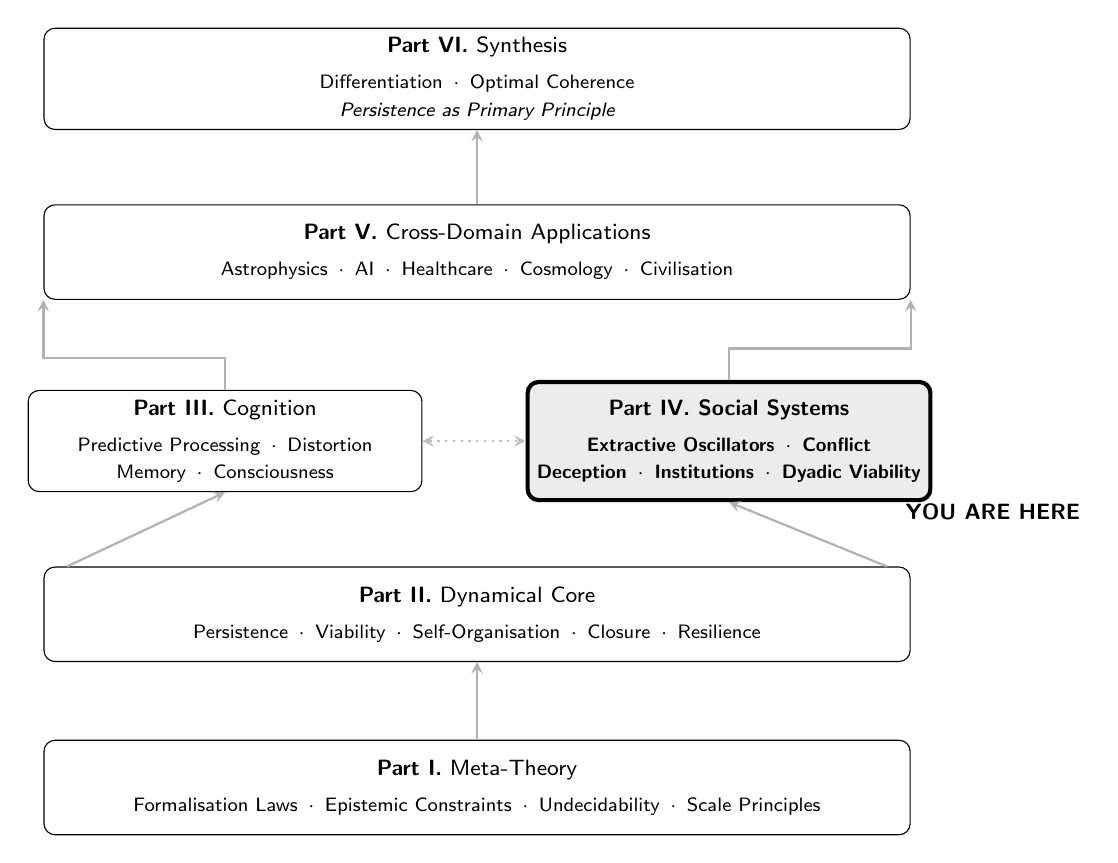
\begin{tikzpicture}[
  every node/.style={font=\sffamily},
  layer/.style={draw, rounded corners=4pt, minimum width=11cm, minimum height=1.2cm, align=center, font=\sffamily\small, fill=white},
  %% --- MOVE "highlight" TO YOUR PAPER'S LAYER ---
  highlight/.style={draw, rounded corners=4pt, minimum width=11cm, minimum height=1.5cm, align=center, font=\sffamily\small\bfseries, fill=gray!15, line width=1.5pt},
  arrow/.style={->, >=stealth, thick, gray!60},
]

% Layer I — Foundation
\node[layer] (meta) at (0, 0) {
  {\footnotesize\textbf{Part I.} Meta-Theory}\\[2pt]
  {\scriptsize Formalisation Laws \,$\cdot$\, Epistemic Constraints \,$\cdot$\, Undecidability \,$\cdot$\, Scale Principles}
};

% Layer II
\node[layer] (core) at (0, 2.2) {
  {\footnotesize\textbf{Part II.} Dynamical Core}\\[2pt]
  {\scriptsize Persistence \,$\cdot$\, Viability \,$\cdot$\, Self-Organisation \,$\cdot$\, Closure \,$\cdot$\, Resilience}
};

% Layer III — Left
\node[layer, minimum width=5cm] (cog) at (-3.2, 4.4) {
  {\footnotesize\textbf{Part III.} Cognition}\\[2pt]
  {\scriptsize Predictive Processing \,$\cdot$\, Distortion}\\[-1pt]
  {\scriptsize Memory \,$\cdot$\, Consciousness}
};

% Layer IV — Right  ← CURRENTLY HIGHLIGHTED (change for your paper)
\node[highlight, minimum width=5cm] (soc) at (3.2, 4.4) {
  {\footnotesize\textbf{Part IV.} Social Systems}\\[2pt]
  {\scriptsize Extractive Oscillators \,$\cdot$\, Conflict}\\[-1pt]
  %% --- CHANGE "Dyadic Viability" TO YOUR PAPER'S SHORT TITLE ---
  {\scriptsize Deception \,$\cdot$\, Institutions \,$\cdot$\, \textbf{Dyadic Viability}}
};

% Marker — move to your layer
\node[font=\sffamily\footnotesize\bfseries] at (6.5, 3.5) {$\blacktriangledown$ YOU ARE HERE};

% Layer V
\node[layer] (app) at (0, 6.8) {
  {\footnotesize\textbf{Part V.} Cross-Domain Applications}\\[2pt]
  {\scriptsize Astrophysics \,$\cdot$\, AI \,$\cdot$\, Healthcare \,$\cdot$\, Cosmology \,$\cdot$\, Civilisation}
};

% Layer VI — Top
\node[layer] (syn) at (0, 9.0) {
  {\footnotesize\textbf{Part VI.} Synthesis}\\[2pt]
  {\scriptsize Differentiation \,$\cdot$\, Optimal Coherence}\\[-1pt]
  {\scriptsize\itshape Persistence as Primary Principle}
};

% Arrows
\draw[arrow] (meta) -- (core);
\draw[arrow] (core.north west) ++(0.3,0) -- (cog.south);
\draw[arrow] (core.north east) ++(-0.3,0) -- (soc.south);
\draw[arrow] (cog.north) -- ++(0, 0.4) -| (app.south west);
\draw[arrow] (soc.north) -- ++(0, 0.4) -| (app.south east);
\draw[arrow] (app) -- (syn);

% Cross-connection
\draw[<->, >=stealth, thick, dotted, gray!50] (cog.east) -- (soc.west);

\end{tikzpicture}
%% --- UPDATE THIS CAPTION FOR YOUR PAPER ---
\caption{Location of the present paper within the Unified Structural Theory of Complex Systems (Kriger, 1999--2026). The theory comprises six layers: foundational meta-theory (I), the dynamical core of structural laws (II), cognitive architecture (III), social systems (IV), cross-domain applications (V), and the overarching synthesis (VI). This paper develops the \emph{Dyadic Viability} model within Part~IV, drawing on the viability, cooperation, and interference laws from Part~II, the structural distortion and extractive oscillator frameworks from Parts~III--IV, and connecting to applications in healthcare, AI, and civilisational analysis in Part~V.}
\label{fig:theory_map}
\end{figure}



% =============================================================
%  APPENDIX D: 76-PAPER PUBLICATION EDIFICE (portrait, 1 page)
% =============================================================
\clearpage
\newgeometry{left=1.2cm, right=1.2cm, top=1.6cm, bottom=0.6cm}

\section*{Appendix D: The Publication Edifice}

\vspace{-1mm}
{\scriptsize All 76 publications (Kriger, 1999--2026) organised bottom-to-top. The present paper is marked~$\blacktriangledown$.}

\vspace{2mm}
\noindent
\resizebox{\textwidth}{!}{%
\begin{tikzpicture}[
  every node/.style={font=\sffamily},
  B/.style={draw, thin, rounded corners=1pt, minimum height=0.6cm, align=left, inner xsep=2pt, inner ysep=1.5pt, font=\sffamily\scriptsize, fill=white, anchor=north west, text width=3.5cm},
  H/.style={draw, line width=1.4pt, rounded corners=2pt, minimum height=0.65cm, align=left, inner xsep=2.5pt, inner ysep=2pt, font=\sffamily\scriptsize\bfseries, fill=black!12, anchor=north west, text width=3.5cm},
  LH/.style={font=\sffamily\scriptsize\bfseries, text=black!45, anchor=south west},
  GA/.style={-{Stealth[length=5pt, width=3.5pt]}, line width=1.4pt, black!30}
]

% 4 columns
\def\cI{0.2}
\def\cII{4.0}
\def\cIII{7.8}
\def\cIV{11.6}
\def\RS{0.88} % row spacing

% ==================================================================
% LAYER I — META-THEORY — 8 papers, 2 rows
% y: 0 to 2.2
% ==================================================================
\fill[black!4, rounded corners=2pt] (0, 0) rectangle (15.3, 2.2);
\node[LH] at (0.1, 2.17) {I\quad META-THEORY};

\node[B] at (\cI,   1.85) {Formalisation Laws (2025)};
\node[B] at (\cII,  1.85) {Imperative Uncertainty (2025)};
\node[B] at (\cIII, 1.85) {Limit to Negation (2025)};
\node[B] at (\cIV,  1.85) {Absurdity as Mercy (2025)};
\node[B] at (\cI,   0.97) {Undecidability as Signal (2023)};
\node[B] at (\cII,  0.97) {No Final Theory: Scale Laws (2024)};
\node[B] at (\cIII, 0.97) {Choice of Formal Realities (2026)};
\node[B] at (\cIV,  0.97) {Def.-Dependent Provability (2026)};

\draw[GA] (7.65, 2.3) -- (7.65, 2.7);

% ==================================================================
% LAYER II — DYNAMICAL CORE — 12 papers, 3 rows
% y: 2.8 to 5.5
% ==================================================================
\fill[black!7, rounded corners=2pt] (0, 2.8) rectangle (15.3, 5.5);
\node[LH] at (0.1, 5.47) {II\quad DYNAMICAL CORE};

\node[B] at (\cI,   5.15) {Four Laws of Self-Org.\ (2017)};
\node[B] at (\cII,  5.15) {Transformational Persistence (2024)};
\node[B] at (\cIII, 5.15) {Structural Resilience (2019)};
\node[B] at (\cIV,  5.15) {Constraint--Autonomy Law (2026)};
\node[B] at (\cI,   4.27) {Viability Mismatch Law (2026)};
\node[B] at (\cII,  4.27) {Newtonian Dynamics Struct.\ (2018)};
\node[B] at (\cIII, 4.27) {Structural Diagnostic Pr.\ (2018)};
\node[B] at (\cIV,  4.27) {Cyclical Hierarchical Syst.\ (2024)};
\node[B] at (\cI,   3.39) {Self-Sufficient Systems (2024)};
\node[B] at (\cII,  3.39) {Assert.--Dismantling Cycles (2015)};
\node[B] at (\cIII, 3.39) {Chaos Is Relative (2026)};
\node[B] at (\cIV,  3.39) {Structural Non-Neutrality (2026)};

\draw[GA] (7.65, 5.6) -- (7.65, 6.0);

% ==================================================================
% LAYER III — COGNITION — 16 papers, 4 rows
% y: 6.1 to 9.7
% ==================================================================
\fill[black!4, rounded corners=2pt] (0, 6.1) rectangle (15.3, 9.7);
\node[LH] at (0.1, 9.67) {III\quad COGNITION};

\node[B] at (\cI,   9.35) {Structural Distortion Pr.\ (2026)};
\node[B] at (\cII,  9.35) {Predictive Processing (2026)};
\node[B] at (\cIII, 9.35) {Representational Isolation (2026)};
\node[B] at (\cIV,  9.35) {Epistemic Constraint Th.\ (2021)};
\node[B] at (\cI,   8.47) {Atemporal Memory (2025)};
\node[B] at (\cII,  8.47) {Evol.\ Sel.\ Atemp.\ Mem.\ (2019)};
\node[B] at (\cIII, 8.47) {Chronoperception Accel.\ (1999)};
\node[B] at (\cIV,  8.47) {Consciousness: Contrad.\ (2021)};
\node[B] at (\cI,   7.59) {Functional Sufficiency (2024)};
\node[B] at (\cII,  7.59) {Operational Term.\ IIT (2024)};
\node[B] at (\cIII, 7.59) {Evol.\ Theory of Credence (2022)};
\node[B] at (\cIV,  7.59) {Reflexive Inference Law (2026)};
\node[B] at (\cI,   6.71) {Mental Disintegration (2026)};
\node[B] at (\cII,  6.71) {Eruptive Manifestation (2026)};
\node[B] at (\cIII, 6.71) {Elim.\ Distortion: Biol.\ Pr.\ (2026)};
\node[B] at (\cIV,  6.71) {Predict.\ Mind: Myth \& Rit.\ (2026)};

\draw[GA] (7.65, 9.8) -- (7.65, 10.2);

% ==================================================================
% LAYER IV — SOCIAL SYSTEMS — 15 papers, 4 rows (4+4+4+3)
% y: 10.3 to 13.9
% ==================================================================
\fill[black!7, rounded corners=2pt] (0, 10.3) rectangle (15.3, 13.9);
\node[LH] at (0.1, 13.87) {IV\quad SOCIAL SYSTEMS};

\node[B] at (\cI,   13.55) {Extractive Oscillators (2017)};
\node[B] at (\cII,  13.55) {Conflict as Phase Trans.\ (2005)};
\node[B] at (\cIII, 13.55) {Deception \& Perc.\ Reality (2025)};
\node[B] at (\cIV,  13.55) {Autonomy Suppression (2020)};
\node[B] at (\cI,   12.67) {Conceptual Responsibility (2014)};
\node[B] at (\cII,  12.67) {Asymm.\ Totalizing Ideals (2026)};
\node[B] at (\cIII, 12.67) {Pre-Integrative Rejection (2026)};
\node[B] at (\cIV,  12.67) {Comparative Asymmetry (2026)};
\node[B] at (\cI,   11.79) {Non-Participation Excl.\ (2026)};
\node[B] at (\cII,  11.79) {Pascal's Wager Dual-Syst.\ (2026)};
\node[B] at (\cIII, 11.79) {Addiction as Extr.\ Osc.\ (2026)};
\node[H] (HERE) at (\cIV, 11.79) {Structural Viability of\\Dyadic Systems (2026)};
\node[B] at (\cI,   10.91) {AI-Extended Communic.\ (2026)};
\node[B] at (\cII,  10.91) {Stimulus Probl.: Post-Sc.\ (2026)};
\node[B] at (\cIII, 10.91) {Inevit.\ Unified Civilis.\ (2026)};

\node[font=\sffamily\small\bfseries, anchor=west] at (15.35, 11.94) {$\blacktriangledown$};

\draw[GA] (7.65, 14.0) -- (7.65, 14.4);

% ==================================================================
% LAYER V — APPLICATIONS — 21 papers, 6 rows
% y: 14.5 to 20.1
% ==================================================================
\fill[black!4, rounded corners=2pt] (0, 14.5) rectangle (15.3, 20.1);
\node[LH] at (0.1, 20.07) {V\quad APPLICATIONS};

\node[font=\sffamily\tiny\itshape, text=black!30, anchor=south west] at (0.2, 19.65) {Astrophysics};
\node[B] at (\cI,   19.55) {Binary-First Star Form.\ (2025)};
\node[B] at (\cII,  19.55) {Why Binary Optimal (2026)};
\node[B] at (\cIII, 19.55) {Swept-Volume Geometry (2026)};
\node[B] at (\cIV,  19.55) {Persist.-Driven Domin.\ (2026)};
\node[B] at (\cI,   18.67) {Protostellar Core Paradox (2026)};
\node[B] at (\cII,  18.67) {Observ.\ Tests VLA/L1551 (2026)};
\node[B] at (\cIII, 18.67) {Can a Star Be Single? (2026)};
\node[B] at (\cIV,  18.67) {Dormant Neutron Stars (2025)};

\node[font=\sffamily\tiny\itshape, text=black!30, anchor=south west] at (0.2, 17.89) {Cosmology \& Methodology};
\node[B] at (\cI,   17.79) {Timescape Cosmology (2025)};
\node[B] at (\cII,  17.79) {Holographic Universe (2025)};
\node[B] at (\cIII, 17.79) {Bayesian Model Comp.\ (2026)};
\node[B] at (\cIV,  17.79) {Struct.-Bayesian Framew.\ (2026)};
\node[B] at (\cI,   16.91) {Ledger Time Model (2025)};

\node[font=\sffamily\tiny\itshape, text=black!30, anchor=south west] at (4.0, 17.13) {Information, AI, Healthcare};
\node[B] at (\cII,  16.91) {Viral Dynamics Framew.\ (2022)};
\node[B] at (\cIII, 16.91) {Quant.\ Clinical Framew.\ (2000)};
\node[B] at (\cIV,  16.91) {Clinical Discont.\ \& AI (2024)};
\node[B] at (\cI,   16.03) {Biospheric Complexity (2026)};
\node[B] at (\cII,  16.03) {Cognitive Syst.\ Compl.\ (2026)};
\node[B] at (\cIII, 16.03) {Local Entropy Inv.\ AI (2026)};
\node[B] at (\cIV,  16.03) {Time Density Dynamics (2026)};
\node[B] at (\cI,   15.15) {Inward Turn: Fermi (2026)};

\draw[GA] (7.65, 20.2) -- (7.65, 20.6);

% ==================================================================
% LAYER VI — SYNTHESIS — 4 papers, 1 row
% y: 20.7 to 21.85
% ==================================================================
\fill[black!7, rounded corners=2pt] (0, 20.7) rectangle (15.3, 21.85);
\node[LH] at (0.1, 21.82) {VI\quad SYNTHESIS};

\node[B] at (\cI,   21.5) {Differentiation as Ontol.\ Cond.\ (2026)};
\node[B] at (\cII,  21.5) {Coherent Syst.\ via Diff.\ (2026)};
\node[B] at (\cIII, 21.5) {Optimal Coherence (2026)};
\node[B] at (\cIV,  21.5) {Inform.\ Preconditions of Meaning (2026)};

% ==================================================================
% APEX
% ==================================================================
\draw[GA] (7.65, 21.95) -- (7.65, 22.35);
\node[draw, thick, rounded corners=3pt, minimum height=0.7cm, align=center, inner sep=5pt,
      font=\sffamily\normalsize\bfseries, fill=black!6, text width=14.8cm, anchor=south west]
  at (0.1, 22.45) {UNIFIED STRUCTURAL THEORY OF COMPLEX SYSTEMS};

\end{tikzpicture}%
}%

\restoregeometry
